\documentclass[a4paper,14pt]{extreport}
\usepackage[left=1.5cm,right=1.5cm,
    top=1.5cm,bottom=1.5cm,bindingoffset=0cm]{geometry}
\usepackage{scrextend}
\usepackage[T1,T2A]{fontenc}
\usepackage[utf8]{inputenc}
\usepackage[english,russian,ukrainian]{babel}
\usepackage{tabularx}
\usepackage{amssymb}
\usepackage{color}
\usepackage{amsmath}
\usepackage{mathrsfs}
\usepackage{listings}
\usepackage{graphicx}
\graphicspath{ {./images/} }
\usepackage{lipsum}
\usepackage{xcolor}
\usepackage{hyperref}
\usepackage{tcolorbox}
\usepackage{tikz}
\usepackage[framemethod=TikZ]{mdframed}
\usepackage{wrapfig,boxedminipage,lipsum}
\mdfdefinestyle{MyFrame}{%
linecolor=blue,outerlinewidth=2pt,roundcorner=20pt,innertopmargin=\baselineskip,innerbottommargin=\baselineskip,innerrightmargin=20pt,innerleftmargin=20pt,backgroundcolor=gray!50!white}
 \usepackage{csvsimple}
 \usepackage{supertabular}
\usepackage{pdflscape}
\usepackage{fancyvrb}
%\usepackage{comment}
\definecolor{ggreen}{rgb}{0.4,1,0}
\definecolor{rred}{rgb}{1,0.1,0.1}
\usepackage{array,tabularx}
\usepackage{colortbl}

\usepackage{varwidth}
\tcbuselibrary{skins}
\usepackage{fancybox}




\usepackage{float}
\usepackage{wrapfig}
\usepackage{framed}
%for nice Code{
\lstdefinestyle{customc}{
  belowcaptionskip=1\baselineskip,
  breaklines=true,
  frame=L,
  xleftmargin=\parindent,
  language=C,
  showstringspaces=false,
  basicstyle=\small\ttfamily,
  keywordstyle=\bfseries\color{green!40!black},
  commentstyle=\itshape\color{purple!40!black},
  identifierstyle=\color{blue},
  stringstyle=\color{orange},
}
\lstset{escapechar=@,style=customc}
%}


\begin{document}
\pagecolor{white}
\begin{titlepage}
  \begin{center}
    \large
    Національний технічний університет України \\ "Київський політехнічний інститут імені Ігоря Сікорського"


    Факультет Електроніки

    Кафедра мікроелектроніки
    \vfill

    \textsc{ЗВІТ}\\

    {\Large Про виконання самостійної роботи №1\\
      з дисципліни: «Схемотехгіка-1»\\[1cm]

      %  Робота з файлами в С++


    }
  \bigskip
\end{center}
\vfill

\newlength{\ML}
\settowidth{\ML}{«\underline{\hspace{0.4cm}}» \underline{\hspace{2cm}}}
\hfill
\begin{minipage}{1\textwidth}
Виконавець:\\
Студент 3-го курсу \hspace{4cm} $\underset{\text{(підпис)}}{\underline{\hspace{0.2\textwidth}}}$  \hspace{1cm}А.\,С.~Мнацаканов\\
\vspace{1cm}

Перевірив: \hspace{6.1cm} $\underset{\text{(підпис)}}{\underline{\hspace{0.2\textwidth}}}$  \hspace{1cm}І.\,П.~Голубєва\\

\end{minipage}

\vfill

\begin{center}
2021
\end{center}
\end{titlepage}


%--------------------------------1-------------------------------
%\begin{center}\fcolorbox{black}{ggreen}{Варіант № 5}\end{center}

\begin{tabularx}{16cm}{|c|c|c|X|X|}
\hline
Варіант & $R_1 $, кОм & $R_2 $, кОм &  Діапазон зміни параметру & Кількість точок по лінійній шкалі\\
\hline
5 & 1 & 6 & \hspace{1.4cm}0...0.2A  & \hspace{1.8cm} 10\\
\hline
\end{tabularx}


\begin{figure}[h]
\begin{center}
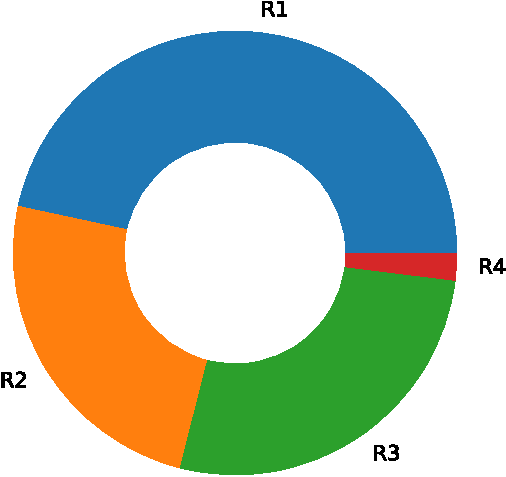
\includegraphics[scale = 0.7]{2.png}
\caption{Схема з номіналами згідно варіанту.}
\label{ris1}
\end{center}
\end{figure}



\begin{center}\textbf{Аналітичні формули для розрахунку струму через резистори $R_1$ та $R_2$} \end{center}

\begin{align}
  I_{R_1} = \dfrac{\dfrac{1}{R_1} }{ \dfrac{1}{R_1} + \dfrac{1}{R_2}} \cdot J \hspace{3cm} I_{R_2} = \dfrac{\dfrac{1}{R_2} }{ \dfrac{1}{R_1} + \dfrac{1}{R_2}} \cdot J ,
\label{q1}
\end{align}
де J -- струм який видає ждерело струму I; R -- опір на резисторі.


\begin{figure}[h]
\begin{center}
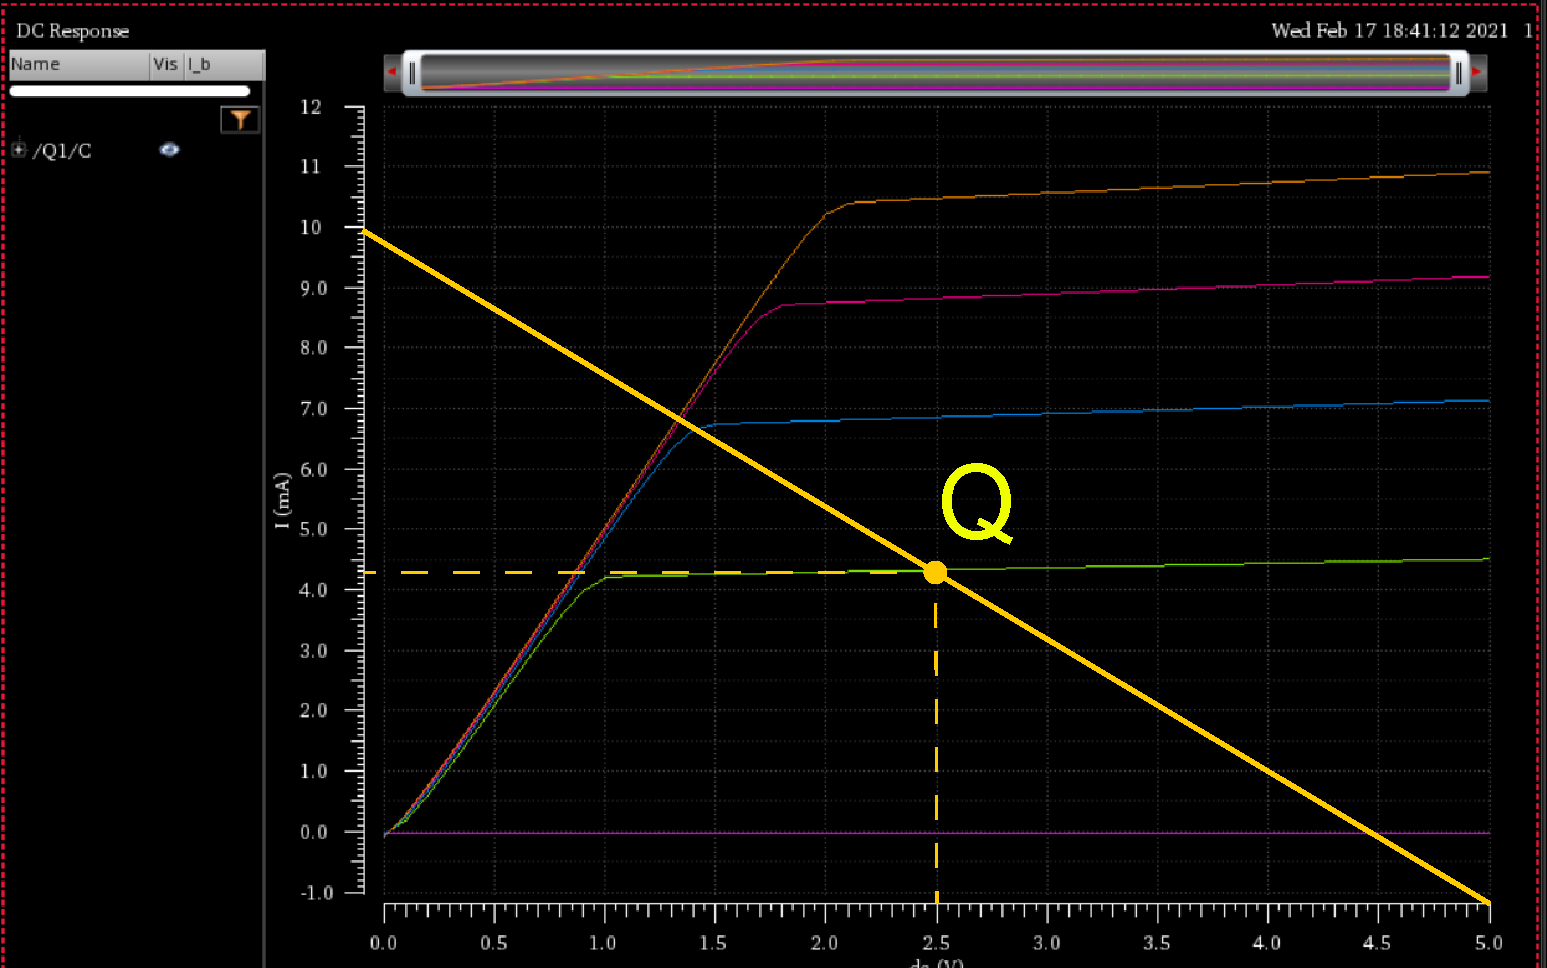
\includegraphics[scale = 0.55]{1.png}
\caption{Графіки із результатами моделювання.}
\label{ris2}
\end{center}
\end{figure}

\newpage
\begin{center}\textbf{Аналіз отриманих результатів} \end{center}

Виконавши параметричний аналіз схеми по постійному струму для схеми дільника
струму рис.(\ref{ris1}) за допомогою редактора схемотехнічних проектів VIRTUOSO та отримав наступні результи, які зоображені на рис.(\ref{ris2}). Підставивши дані в формули для роздахунку струмів на резисторах (\ref{q1}), отримав що $I_{R_1} \approx 0.85\cdot J$  та $I_{R_2} \approx 0.14 \cdot J$ і таким чином переконався у тому що отримані результати задовольняють вищезгадані формули.








\end{document}
